\documentclass[12pt,a4paper]{article}
\usepackage{textcomp}
\usepackage[latin1]{inputenc}
\usepackage[T1]{fontenc}
\usepackage{lmodern}
\usepackage{amsmath}
\usepackage{amsfonts}
\usepackage{amssymb}
\usepackage{amsthm}
\usepackage{color}
\usepackage{graphicx}
\usepackage{hyperref}
\usepackage[ruled,vlined]{algorithm2e}
\newtheorem{thm}{Theorem}
\definecolor{gris25}{gray}{0.80}
\newcommand{\encadre}[1]{\fcolorbox{black}{gris25}{\begin{minipage}{1.0\textwidth}\medskip #1 \vspace{0.1pt}\end{minipage}}}
\newtheorem{prop}[thm]{Property}
\newtheorem{lem}[thm]{Lemme}
\newtheorem{cor}[thm]{Corollaire}
\newtheorem{hyp}[thm]{Hypothesis}
\def\N{{\mathbb{N}}}
\def\R{{\mathcal{R}}}
\newcommand\independent{\protect\mathpalette{\protect\independenT}{\perp}}
\def\independenT#1#2{\mathrel{\rlap{$#1#2$}\mkern2mu{#1#2}}}

\title{\textsc{Degree Project} \\
\large{\textbf{Measuring association between heterogeneous time-series}}}

\author{Alexandre GUINAUDEAU\\
\href{mailto:alegui@kth.se}{alegui@kth.se}\\
\\
Supervisor: Pawel Herman\\
\\
Examiner: Hedvig Kjellstr{\"o}m\\
}

\date{\today}

\begin{document}

\maketitle

\newpage

\tableofcontents

\newpage

\section*{Introduction}
\label{sec:intro}
\addcontentsline{toc}{section}{\nameref{sec:intro}}

As it spreads to many industries and increases in volume, sensor data is a becoming an important field of research in terms of security, storage, and analysis.
In manufacturing plants, aircrafts, electronic intensive care units or data centers, sensors continuously monitor many parameters of the environment.
The data generated by these sensors is then processed to optimize the way the system works, or to diagnose failures once they occurred.
These systems can have hundreds or thousands of sensors with sub-second sampling.
With this amount of data, diagnosing failures requires an efficient processing of the data.\\

Finding other data that is associated with the failures and can contribute to explaining them is critical to understand the circumstances of the incident and troubleshoot it.
In most cases, the cause of the failures is specific to what the data represents.
For instance, the sensor data could be a consequence of the failure rather than a cause, or a third factor could have affected both the sensor and the system.
In any case, providing the system engineer with a limited list of sensors that seem to have some correlation with the failure is very valuable to enable them to quickly troubleshoot the problem.
Once the engineers know where to look, they are usually able to understand what happened by diving into the specific environment parameters.

\paragraph{Interest and assignment}

The main difficulty to solve this problem is the heterogeneity of the data: it can be continuous data (for instance measures of environment parameters such as a pressure or a temperature), categorical data (for instance the part that is installed on a machine) or events (for instance when an operation is triggered). In many cases a time series can be represented in all of these ways, but in general one of them makes more sense.

In this thesis we do not care whether the one time series is the cause of the other, nor whether there is a positive or linear correlation between them. We only care about is a generalization of the \emph{association} of binary variables, more precisely whether the knowledge of one times series can improve the understanding of the other one.

\medskip

\textbf{When can a continuous or categorical time series be considered as associated to a binary event time series? More specifically, what metric can be defined to measure association between heterogeneous time series?}

\medskip

I have access to a large set of real data - both sensor and event data. However, given the sensitivity of this data, I will use other data for this report.
I will generate fake data, starting with examples based on simple probability rules to understand how correlation metrics work and how they can be generalized. Then I will use notional data from open source examples or generated in a real environment, to confirm the hypothesis scale to real-life examples.

\clearpage

\section{Pilot study}

\subsection{News value}

Automatically finding associated sensor time series would be very valuable for all of the systems described above to troubleshoot failures faster and anticipate them. 
It could be applied to any system that has a logging system generating frequent debug messages and a few error events independently.
Microsoft researched suggested a solution to correlate continuous and event time series \cite{incident-diagnosis} but focused more on the temporal correlation - so the causal correlation - rather than the actual association between timeseries. For non-stationary time series, we assume they have been transformed to be stationary - or more exactly, we will show some ways to transform stationary timeseries to stationary ones.

% My thesis is motivated by a real-world application of incident diagnosis.

\subsection{Correlation metrics}
The most common metric to measure correlation is the \emph{Pearson} coefficient. It can easily be interpreted and visualized \cite{pearson}, and often gives very good results. However, in some case, it can be misleading, especially because it only captures linear correlations and because it assumes normal distribution of the input parameters.

In this case, the \emph{Spearman} coefficient is more robust (although less efficient), as it only compares ranks between elements, and therefore captures monotonic correlations, even if there are not linear. The \emph{Kendall} coefficient is very similar as it also uses the rank of elements to compare them, it is less efficient but more robust. It is also much easier to interpret, as it captures the percentage of elements positively correlated \cite{spearman-kendall, spearman-kendall2}. These correlation metrics are probably more adapted to our problem for numerical data as they capture non-linear correlations, but may be harder to generalize because their definition is not as simple as Pearson's.

\subsection{Association metrics}

All these usual correlation metrics apply to numerical data, and cannot therefore be used for categorical data. In this case, a metric that often works well is the J-measure \cite{j-measure-rule, j-measure}, which is based on the concept of entropy in information theory. For binary data, it is possible to transform the data to make most association measures equivalent \cite{metric-comparison}. This is not as clear for more complex data, and requires to clearly define the concept of association for categorical and continuous data as well.

However, it is not clear if this measure can be compared to the previous ones when the data is both numerical and categorical - for instance when it is binary. In \cite{metric-comparison}, P-N Tan et al. compared many existing norms on binary classification, and showed their was a way to normalize the data in order to make all the norms they studied equivalent. Such techniques will be important to pre-process the data accurately and to generalize norms to heterogeneous time series.

\subsection{Application to heterogeneous data}
Several tools exist to analyze the correlation between continuous time series \cite{tool-continuous}, or between events \cite{tool-event3}, but they do not perform well when it comes to correlating continuous time series and events. However, sensor data is heterogeneous: it can be continuous, discrete, categorical or binary.
Usual measures of correlation such as the Pearson and Spearman correlation do not perform well on this kind of data \cite{incident-diagnosis}.
Therefore, we have to find other ways of defining association. We can also map continuous or categorical time series to event time series - by detecting outliers or change points - and apply existing tools to the transformed data \cite{categorical-time-series, detect-change-points}.

\newpage

\section{Defining association for heterogeneous time series}

In order to find time series which can help us troubleshoot failures, we must first define \emph{association} in a clear way. 
To do so, we will define a set of properties that a good association metric should abide by, and then define very simple examples where we know how the association metric should behave. 
Then, we will compare candidate metrics based on these properties and examples in order to select the ones that correctly measure association.

\subsection{Fundamental properties}
\label{sec:properties}

\subsubsection{Notations and definitions}

Given two time series $x$ and $y$, we note $A(x, y)$ the association between them. Without loss of generality, we can assume that our metric gives a score from 0 to 1.

$x$ and $y$ are associated if the knowledge of one improves the understanding of the other, in other words if the posterior model forecasts values better than the prior model.
More formally, we note $\mathcal{P}(x_t | x_0, \ldots, x_{t-1})$ the forecast of $x_t$ at the instant $t$, given all previous observations, and $\mathcal{P}_y(x_t | x_0, \ldots, x_{t-1})$ the forecast of $x_t$ at the instant $t$ given all previous observations of $x$ and all observations of $y$.

We also define a loss metric $\mathcal{L}$ which measures the surprise:

$$\mathcal{L}(x)_t = dist(\mathcal{P}(x_t | x_0, \ldots, x_{t-1}), x_t)$$
$$\mathcal{L}(x|y)_t = dist(\mathcal{P}_y(x_t | x_0, \ldots, x_{t-1}), x_t)$$

where $dist$ is a distance metric. 

\subsubsection{Properties}

With these notations, a good metric to measure association between time series should follow the following properties:\\

\noindent
\fbox{
    \parbox{\textwidth}{%
\begin{enumerate}
    \vspace{-.5em}
    \item[\textbf{P1.}] \textbf{(Independence)} $A(x, y) = 0 \Leftrightarrow x \independent y$
    \item[\textbf{P2.}] \textbf{(Information gain)} $ A(x, y) > 0 \Leftrightarrow \mathcal{L}(x | y) < \mathcal{L}(x)$
    \item[\textbf{P3.}] \textbf{(Perfect knowledge)} $A(x, y) = 1 \Leftrightarrow \mathcal{L}(x | y) = 0$
    \item[\textbf{P4.}] \textbf{(Symmetry)} $A(x, y) = A(y, x)$: $A$ should be symmetric
    \vspace{-.5em}
\end{enumerate}
    }%
}

\subsection{Expected behavior for simple examples}
\label{sec:simple_examples}

We also define simple examples where we can know how the association should behave.

\subsubsection{Categorical and event data}

Our first example compares an event time series and a categorical one. This could for instance be useful to determine whether an installed part tends to fail more often than another. We will start with the case of two categories and then generalize to any number of categories.
Let $x$ be a time series of events, that occur with probability $p_1$ during $t_1$ and then at frequency $p_2$ during $t_2$. Let $t_{tot} = t_1 + t_2$ the total time, 
$p_{tot} = \frac{p_1 n_1 + p_2 n_2}{n_1+n_2}$ the average probability of failure. Let $y$ be a categorical time series with value $C_1$ during $t_1$ and $C_2$ during $t_2$. 

\begin{figure}[h]
\centering
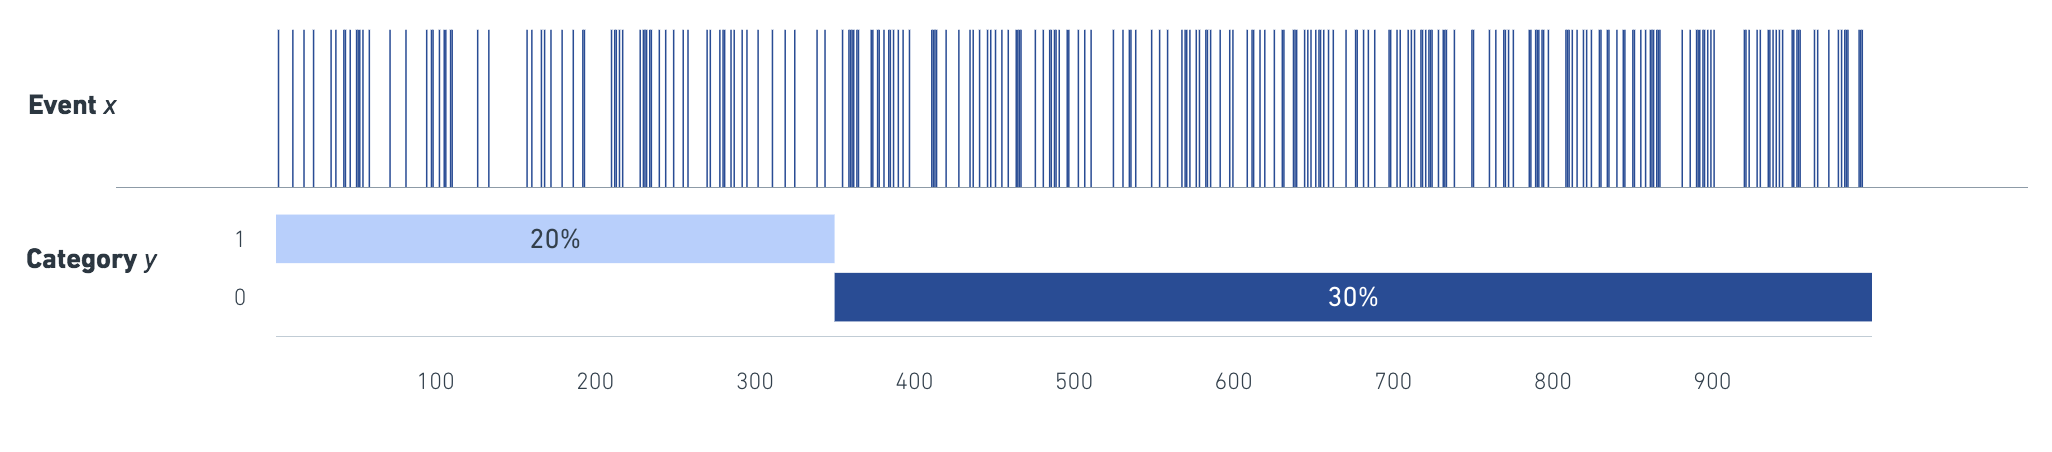
\includegraphics[width=\textwidth]{categorical_event_series}
\caption{Example of associated categorical and event series}
\label{fig:categorical_event_series}
\end{figure}

Figure \ref{fig:categorical_event_series} shows an example of such time series $x$ and $y$.
Let's consider other candidate time series $y_k$ with value $C_1$ during $t_1'=k$ and $C_2$ during $t_2'=t_{tot}-k$. 
A good association metric should rank $y_i$ time series such that $y_{t_1}$ has the highest association with $x$. 

\subsubsection{Numerical and event data}

For numerical data, we cannot expect to have a metric that computes the association in the right way on any raw dataset, because the association depends on what the data represents. 
Events can be triggered by extreme values or by sudden changes, they can depend on the original value, or on the de-trended or de-seasoned value. 
Events could also have an impact in the future, or for a specific duration. 
Therefore, we assume the data is preprocessed (potentially de-trended, de-seasoned, shifted, smoothed, derived, normalized) such that large values have a higher risk of triggering an event. 
This is not a real loss of generality, because one can derive multiple preprocessed series out of the original one, for instance using all the methods described above, and the algorithm will only find candidates with high association with the event series.

Let $x$ be a time series of events, and $y \sim \mathcal{N}(0, \sigma)$ be a series of Gaussian white noise, which could be for instance the residual of a de-seasoned and de-trended series. When an event occurs, $y$ has a higher value in average:

$$
y \sim \left\{
\begin{array}{ll}
\mathcal{N}(0, \sigma) & if\ x = 0 \\
\mathcal{N}(1, \sigma) & if\ x = 1
 \end{array}\right.
$$

In this case, we expect $x$ and $y$ to be highly associated. Furthermore, if we define other numerical series that are impacted by a fraction of the events, or by additional events, they should have a lower association with $x$.

\begin{figure}[h]
\centering
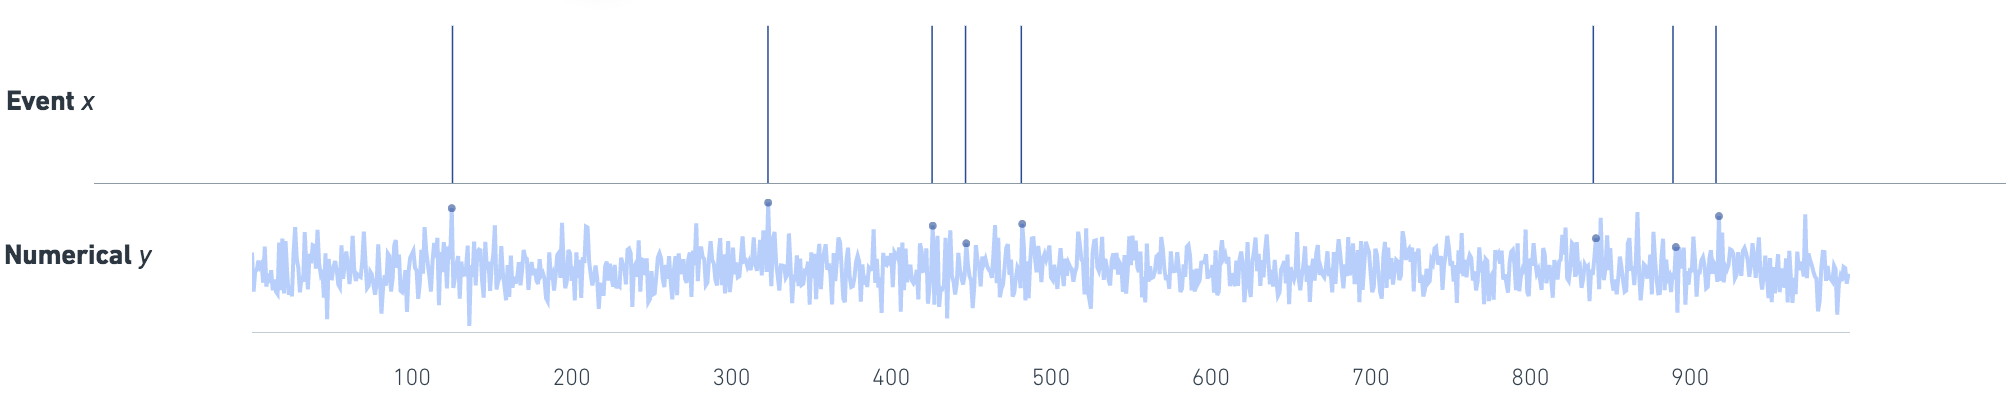
\includegraphics[width=\textwidth]{numerical_event_series}
\caption{Example of associated numerical and event series ($\sigma = 0.4$)}
\label{fig:numerical_event_series}
\end{figure}

Figure \ref{fig:numerical_event_series} shows and example of such series $x$ and $y$. 
Let's consider other numerical time series $y_k$ having larger values for either a subset or a superset of the events $x$. A good association metric should rank these time series such that $y$ has the highest association with $x$.


\subsection{Comparison of different metrics}

We will start by studying usual metrics that could capture the association between time series. We will compare them based on the properties and examples defined in sections \ref{sec:properties} and \ref{sec:simple_examples}, and see how they can be generalized to apply to any time series.

\subsubsection{Pearson Correlation Coefficient}
The most common measure of correlation is the one defined by Pearson $\rho$ defined by:

$$
\rho_{x,y} = \frac{cov(x, y)}{\sigma_x \sigma_y} =  \dfrac{\sum_i (x_i - \overline{x}) (y_i - \overline{y})}{\sqrt{\sum_i (x_i - \overline{x})^2} \sqrt{\sum_i (y_i - \overline{y})^2}}
$$

To capture both correlated and anti-correlated time series we consider its square value $\rho^2$. 

\paragraph{Properties}
It verifies all implications ($\Rightarrow$) of the above properties: a high Pearson correlation coefficient indicates that the knowledge of a series increases our knowledge of the other. However, it only captures linear correlation, so we could miss association between series with non-linear correlation (\textbf{P2.} $\nLeftarrow$ and \textbf{P3.} $\nLeftarrow$). 

\paragraph{Categorical data}
In order to compute the Pearson correlation coefficient for the first example, we need the categorical data to have numerical values, we set $C_1 = 1$ and $C_2 = 0$.
%TODO Add plot of good correlation

\paragraph{Numerical data}
For the second example, the correlation score will be quite low even when there is a high association because the correlation is not linear. While the series are correctly ranked, the value of the correlation is hard to interpret and does not indicate how significant the association is.


\subsubsection{Spearman and Kendall Correlation Coefficients}

Spearman and Kendall both defined correlation metrics based on the ranking of elements rather than their exact value. 

The Spearman coefficient is the Pearson correlation between the ranks of the elements in $x$ and $y$, which for series with distinct elements is equivalent to:
$$r_s = 1 - \dfrac{6 \sum_i (rank(x_i) - rank(y_i))}{t (t^2 - 1)}$$

The Kendall coefficient computes the proportion of pairs $(i, j)$ for which both series have a concordant order $x_i > x_j$ or $x_i < x_j$:
$$\tau = \dfrac{1}{t (t-1)}\sum_{i \neq j} sgn(x_i - x_j) sgn(y_i - y_j)$$

\paragraph{Properties}

While these two coefficients capture non-linear correlations, they still do not capture non-monotonous correlation, for instance if extreme values of $x$ (positive or negative) correspond to high values of $y$ (\textbf{P2.} $\nLeftarrow$ and \textbf{P3.} $\nLeftarrow$). 

\paragraph{Categorical data}

In the first case, Spearman and Kendall correlations are equivalent to Pearson correlation because both series can only take 2 different values, so sorting them gives the same result as taking their absolute value.

\paragraph{Numerical data}
In the second case however, these coefficients give different results than the Pearson coefficient. They can give better results because they capture non-linear correlations, but might miss the distinction between outliers and relatively high values.
They will bias towards series that are impacted by few events, as they will consider the association to be perfect if the events $x$ correspond exactly to the largest values of $y$.

These two coefficients are interesting to consider in addition to the Pearson coefficient as they capture other kinds of correlations, but they are also hard to interpret and could miss some obvious associations.

\subsubsection{Null hypothesis}

\paragraph{Properties}

%TODO

\paragraph{Categorical data}

We can formulate the examples as null hypothesis problems.
For the first example, the null hypothesis is:

\vspace{1em}
\medskip
\noindent
\fbox{
    \parbox{\textwidth}{%
    \vspace{-1em}
\center $H_0$: Events in the time intervals $[0, t_1]$ and $[t_1, t]$ \\

were drawn with the same probability $p$
    }%
}
\medskip

The z-test associated with this hypothesis is
$$Z = \frac{p_1-p_2}{\sqrt{p(1-p)\left(\frac{1}{t_1}+\frac{1}{t_2}\right)}}$$

We reject the null hypothesis if $Z > \alpha$. We note that $Z$ is proportional to the Pearson factor as $Z = \sqrt{t_{tot}}*\rho$. 

\paragraph{Numerical data}
For the second example, a hypothesis we could refute is that both groups (the values of $y$ when $x$ occurs and its values when $x$ does not occur) were drawn from the same distribution. This should give good results but requires a prior kind of distribution to be defined, in this case we can consider :

\vspace{1em}
\medskip
\noindent
\fbox{
    \parbox{\textwidth}{%
    \vspace{-1em}
\center $H_0$: $y_{|x=1}$ and $y_{|x=0}$ were drawn from the same distribution $\mathcal{N}(\mu, \sigma)$
    }%
}
\medskip

The z-test associated with this hypothesis is
$$Z = \frac{\mu_1-\mu_2}{\sigma}\sqrt{t_{tot}}$$

where $\mu_1$ and $\mu_2$ are the average values of $y_{|x=1}$ and $y_{|x=0}$ respectively.\\

In both cases, the null hypothesis definition requires a prior knowledge of the data, but gives us a good way to interpret the association score. For instance, when $Z > \alpha_{0.99}$, we can reject the null hypothesis with 99\% confidence, in other words the probability of occurrence if very likely to have changed at some point.

\paragraph{Mutual Information}

When considering categorical data, measures of association usually involve the information entropy. The metric that measures shared entropy is the mutual information. For categorical or discrete data, the mutual information is defined by

$$I_{x,y} = H_x + H_y - H_{x, y} = \sum_i \sum_j p(x_i, y_j) \log \left( \dfrac{p(x_i, y_j)}{p(x_i) p(y_j)} \right)$$

where $H$ denote the entropies and $p$ denotes probabilities. More specifically $p(x,y)$ is a joint probability function, and $p(x)$ and $p(y)$ are marginal probability distribution functions.

Its definition can be generalized to continuous data (see \ref{appendix}):

The mutual information is 
$$I = H_1 + H_2 - H_{tot}$$
where $H_{i} = -t_{i} \left(p_{i} \log p_{i} + (1-p_{i}) \log(1-p_{i})\right)$

\paragraph{Properties}

\paragraph{Categorical data}

\paragraph{Numerical data}

\subsubsection{Conclusion}

%\begin{table}[]
%\centering
%\caption{My caption}
%\label{my-label}
%\begin{tabular}{lllll}
%Metric                            & Properties &Categorical & Numerical & Interpretability & Generalizable \\
%Pearson                         & No             & Yes            &                    & No                     & No \\
%Spearman and Kendall & No             & Yes            &                    & No                     & No  \\
%Null hypothesis             & Yes           & Yes            &                    & Yes                    & No \\
%Mutual Information       & Yes           & Yes            &                    &                            & Yes
%\end{tabular}
%\end{table}




\subsubsection*{Ranking candidate time series}

%TODO Add
\paragraph{Theory}
Let's consider other candidate time series $y_i$ with value $C_1$ during $t_1'$ and $C_2$ during $t_2'=t_{tot}-t_1'$. 
A good association metric should rank $y_i$ time series such that $y_{t_1}$ has the highest association with $x$. 
In this example, all metrics studied here find the same optimal associated time series in theory, because $p_1'-p_2'$ decreases for values of $t_1'$ close to $t_2'$, and $\dfrac{1}{t_1'}$ or $\dfrac{1}{t_2'}$ is very large for extreme values of $t_1'$, so $z' < z$.

\paragraph{Practice}
In practice, we used the Monte-Carlo method to compute the error between the expected best candidate and the actual one. We note that results are pretty good, even for small differences between $p_1$ and $p_2$ where it's even hard for a human eye to detect the change in probability. The main bias is towards extreme values of $t_1'$, when the random samples had an unusually high (or low) frequency at the beginning or at the end. However, using the Null Hypothesis method we can ignore the best candidate when the hypothesis is rejected, in which increases the accuracy of the model.

\section{Application to real data}

\subsection{Preprocessing}

%TODO Move to preprocessing
\subsubsection*{Generalization}
We can generalize the results above to any categorical data, and to events with any number of change of frequency. Using the null hypothesis, we can recursively split the event time series into phases where the frequency of occurrence is statistically constant. This can be used to preprocess event time series.
The mutual information formula remains valid for any number of categories. It biases towards many categories, as the mutual information is always strictly positive. To balance this, we could penalize the mutual information such as defined in [A penalized mutual information criterion for blind separation of convolutive mixtures Mohammed El Rhabi, Guillaume Gelle, Hassan Fenniri, Georges Delaunay]. To keep our algorithm efficient enough to compare thousands of sub-second time series, we decided not to penalize the mutual information.

\subsection{Data}

\subsection{Results}

\section*{Conclusion}

\newpage

\section*{Appendix}
\label{sec:appendix}
\addcontentsline{toc}{section}{\nameref{sec:appendix}}

\setcounter{section}{0}
\renewcommand\thesection{\Alph{section}}
\section{Mutual information generalization}\label{appendix}

We use Kraskov et al.'s idea \cite{estimating-mutual-information} to estimate the mutual information between numerical time series drawn from an unknown distribution. If we used the same definition as for discrete data, we would systematically have a mutual information of 1, because no pair of point would have exactly the same value, so the knowledge of a time series would enable us to know the value of the other one. However, this behavior is not expected, as learning these correlation 

%TODO Define better the loss for time series, based on past values but using future value of the other one.

The previous definition of mutual information was defined for categorical data. For numerical data, the joint probability of two variables is also well defined if the underlying distribution is known:

[insert formula here]

However, it is possible to approximate this underlying distribution by considering the $k$-nearest neighbors of each point. Given $k$, for each point $P$, we compute the distance $\varepsilon$ to its $k$-nearest neighbor. If the underlying distribution $\mu$ was uniform, then the probability of being in the ball of center $P$ and of diameter $\varepsilon$ would be $\mu \times V$, where $V$ is the volume of this ball. By deriving this expression, we get an approximation of the entropy:

[insert here]

And by extension of the mutual information between two numerical series. This expression is only valid for numerical data where all values are different (or at least where there are never more than $k-1$ elements with the same value), which can be circumvented by adding a small random noise.

\clearpage

% \tableofcontents


\begin{thebibliography}{9}
% Climate
\bibitem{climate}
Claude Frankignoul, Klaus Hasselmann (1977) \\
\textit{Stochastic climate models, Part II - Application to sea-surface temperature anomalies and thermocline variability},
Tellus, 29:4, 289-305\\
% \url{https://doi.org/10.3402/tellusa.v29i4.11362}

% Categorical Time series
\bibitem{categorical-time-series}
David S. Stoffer, David E. Tyler, Andrew J. McDougall (1993)\\
\textit{Spectral Analysis for Categorical Time Series: Scaling and the Spectral Envelope},
Biometrika Vol. 80, No. 3, pp. 611-622\\
% \url{https://www.researchgate.net/profile/David_Tyler2/publication/239726763_Spectral_Analysis_for_Categorical_Time_Series_Scaling_and_the_Spectral_Envelope/links/0046352d842c990d8d000000.pdf}

% distance-based outliers
\bibitem{pearson}
Joseph Lee Rodgers and W. Alan Nicewander (1987)\\
\textit{Thirteen Ways to Look at the Correlation Coefficient}, pp 59-66
Download citation  https://doi.org/10.1080/00031305.1988.10475524

\bibitem{j-measure-rule}
Smyth, P. and Goodman, R.M. (1992)\\
\emph{An Information Theoretic Approach to Rule Induction from Databases}, IEEE Transactions on Knowledge and Data Engineering, 4 (Aug. 1992), 301-316

\bibitem{spearman-kendall}
Valz P.D. \& Thompson M.E. (1994) \\
\textit{Exact inference for Kendall's
S and Spearman's rho}, Journal of Computational and
Graphical Statistics 3: 459-472.

\bibitem{anomaly-1}
E. M. Knorr and R. T. Ng. (1998)\\
\textit{Algorithms for Mining Distance-Based Outliers}, In Proceedings of the 24th
International Conference on Very Large Databases (VLDB), pages 392-403, 1998.\\
% \url{http://www.vldb.org/conf/1998/p392.pdf}

\bibitem{j-measure}
Goodman, R.M. and Smyth, P. (1998)\\
\emph{An information-theoretic model for rule-based expert systems}, Int. Symposium in Information Theory, Kobe, Japan, 1988

% Iterative partitioning of time segments to detect change points
\bibitem{detect-change-points}
Valery Guralnik, Jaideep Srivastava (1999)\\
\textit{Event Detection from Time Series Data}, In Proceedings of the Fifth ACM SIGKDD International Conference on Knowledge Discovery and Data Mining (KDD'99), pp. 33-42, August 15-18, 1999, San Diego, CA, USA. \\
% \url{http://dmr.cs.umn.edu/Papers/P1999_6.pdf}

% Different kinds of sensors:
% Intensive Care Unit => alerts based on hardcoded thresholds
\bibitem{icu}
M.-C. Chambrin, P. Ravaux, D. Calvelo-Aros, A. Jaborska, C. Chopin, B. Boniface (1999)\\
\textit{Multicentric study of monitoring alarms in the adult intensive care unit (ICU): a descriptive analysis},
Intensive Care Medicine, Volume 25, Issue 12, pp 1360-1366\\
% \url{https://doi.org/10.1007/s001340051082}

\bibitem{anomaly-2}
S. Ramaswamy, R. Rastogi, and K. Shim. (2000)\\
\textit{Efficient algorithms for mining outliers from large data sets}, In
SIGMOD '00: Proceedings of the 2000 ACM SIGMOD international conference on Management of
data, pages 427-438, 2000.
% \url{https://dl.acm.org/citation.cfm?id=335437&dl=ACM&coll=DL&CFID=841695128&CFTOKEN=52089307}

\bibitem{lof}
M. M. Breunig, H. Kriegel, R. T. Ng, and J. Sander (2000)\\
\textit{LOF: Identifying density-based local outlier}
In Proceedings of the ACM SIGMOD International Conference on Management of Data, pages 93-104, 2000\\
% \url{http://www.dbs.ifi.lmu.de/Publikationen/Papers/LOF.pdf}

% \bibitem{multilevel-surprise}
% C. Shahabi, X. Tian, and W. Zhao. TSA-tree (2000)\\
% \textit{A wavelet-based approach to improve the efficiency of multilevel surprise and trend queries on time-series data},
% In Statistical and Scientific Database Management, pages 55-68, 2000.\\
% \url{https://infolab.usc.edu/DocsDemos/pakdd01.pdf}

\bibitem{global-local-outliers}
C.Shahabi, S. Chung, M.Safar and G.Ha jj (2001)\\
\textit{2D TSA-tree: A Wavelet-Based Approach to Improve the Efficiency of Multi-Level Spatial Data Mining},
Technical Report 01-740, Department of Computer Science, University of Southern California. (2001)\\
% \url{https://pdfs.semanticscholar.org/39c5/5ee09a2c49e736de730e2cc7cc61f789ace1.pdf}
% Tree splitting each signal in 2, a low-pass and a high-pass signal – Detect global outlier regions and local outliers within regions

\bibitem{anomaly-3}
F. Angiulli and C. Pizzuti. (2002)\\
\textit{Fast outlier detection in high dimensional spaces},In PKDD '02: Proceedings
of the 6th European Conference on Principles of Data Mining and Knowledge Discovery, pages 15-26,
2002
% \url{https://link.springer.com/chapter/10.1007/3-540-45681-3_2}

% Multiscale timeseries + multiscale entropy (Computed for several down-samples of the original timeseries)
\bibitem{multiscale-timeseries}
Costa M, Goldberger AL, Peng CK (2002)\\
\textit{Multiscale entropy analysis of complex physiologic time series},
Phys Rev Lett 2002, 89: 068102. 10.1103/PhysRevLett.89.068102\\
% \url{https://dbiom.org/files/publications/Peng_MultiscaleEntropyAnalysisComplexPhysiologicTimeSeries.pdf}

\bibitem{metric-comparison}
Pang-Ning Tan*, Vipin Kumar, Jaideep Srivastava (2004)\\
\textit{Selecting the right objective measure for association analysis}

\bibitem{estimating-mutual-information}
Alexander Kraskov, Harald Stögbauer, and Peter Grassberger (2004)\\
\textit{Estimating mutual information}, 
Phys. Rev. E 2004, 69: 066138. 10.1103/PhysRevE.69.066138\\

% % Parameter-free clustering of similar time series
% \bibitem{parameter-free-clustering}
% Keogh, E., Lonardi, S., Ratanamahatana, C. (2004)\\
% \textit{Towards Parameter-Free Data Mining},
% In proceedings of the 10th ACM SIGKDD International Conference on Knowledge Discovery and Data Mining.\\
% \url{http://www.cs.ucr.edu/~eamonn/SIGKDD_2004_long.pdf}

\bibitem{detecting-anomalies}
Umaa Rebbapragada, Pavlos Protopapas, Carla E. Brodley, Charles Alcock (2009)\\
\textit{Finding anomalous periodic time series}
Machine Learning, v.74 n.3, p.281-313, March 2009. doi: 10.1007/s10994-008-5093-3\\
% \url{https://arxiv.org/pdf/0905.3428.pdf}

\bibitem{spearman-kendall2}
Xu Weichao, Yunhe Hou, Hung Y. S. \& Yuexian Zou (2010)\\
\textit{Comparison of Spearman's rho and Kendall's tau in normal and contaminated normal models}, Manuscript submitted to IEEE Transactions on Information Theory\\
% \url{http://arxiv.org/PS_cache/arxiv/pdf/1011/1011.2009v1.pdf}

\bibitem{tool-event3}
 J.-G. Lou, Q. Fu, Y. Wang, and J. Li (2010)\\
\textit{Mining dependency in distributed systems through unstructured logs analysis}, SIGOPS Operating Systems Review, 41(1):91-96, 2010.

\bibitem{tool-continuous}
D. Wu, Y. Ke, J. X. Yu, S. Y. Philip, and L. Chen (2010)\\
\textit{Detecting leaders from correlated time series}, In Database Systems for Advanced Applications, pages 352-367. Springer.

\bibitem{incident-diagnosis}
Zhang, Dongmei and Lou, Jian-Guang and Ding, Justin and Fu, Qiang and Lin, Qingwei (2014)\\
\textit{Correlating Events with Time Series for Incident Diagnosis},
SigKDD'14, July 2014\\
% \url{https://www.microsoft.com/en-us/research/publication/correlating-events-time-series-incident-diagnosis-2/}


% % Down-sampling time-series and measuring information lost
% \bibitem{downsampling}
% H. Cui, K. Keeton, I. Roy, K. Viswanathan, and G. R. Ganger (2015)\\
% \textit{Using data transformations for low-latency time series analysis},
% In Proceedings of the Sixth ACM Symposium on Cloud Computing, pages 395-407. ACM, 2015\\
% \url{https://www.labs.hpe.com/techreports/2015/HPL-2015-74.pdf}

\end{thebibliography}


\end{document}
